\chapter{Code Quality}
\label{appendix:code_quality}

The BetterCodeHub\footnote{\url{https://bettercodehub.com/}} platform was used for tracking the code quality for our code. In Figure \ref{fig:code_quality} we show the metrics generated after running the analysis on our code base. The separate concerns in modules guideline is violated since we chose to have a common abstract class, implemented by all our other rules, which holds most of the common functionality for parsing the queries. This was preferred since it makes it easier for adding new rules in the future as well as making it easier for testing the rules.

\begin{figure}[ht]
    \centering
    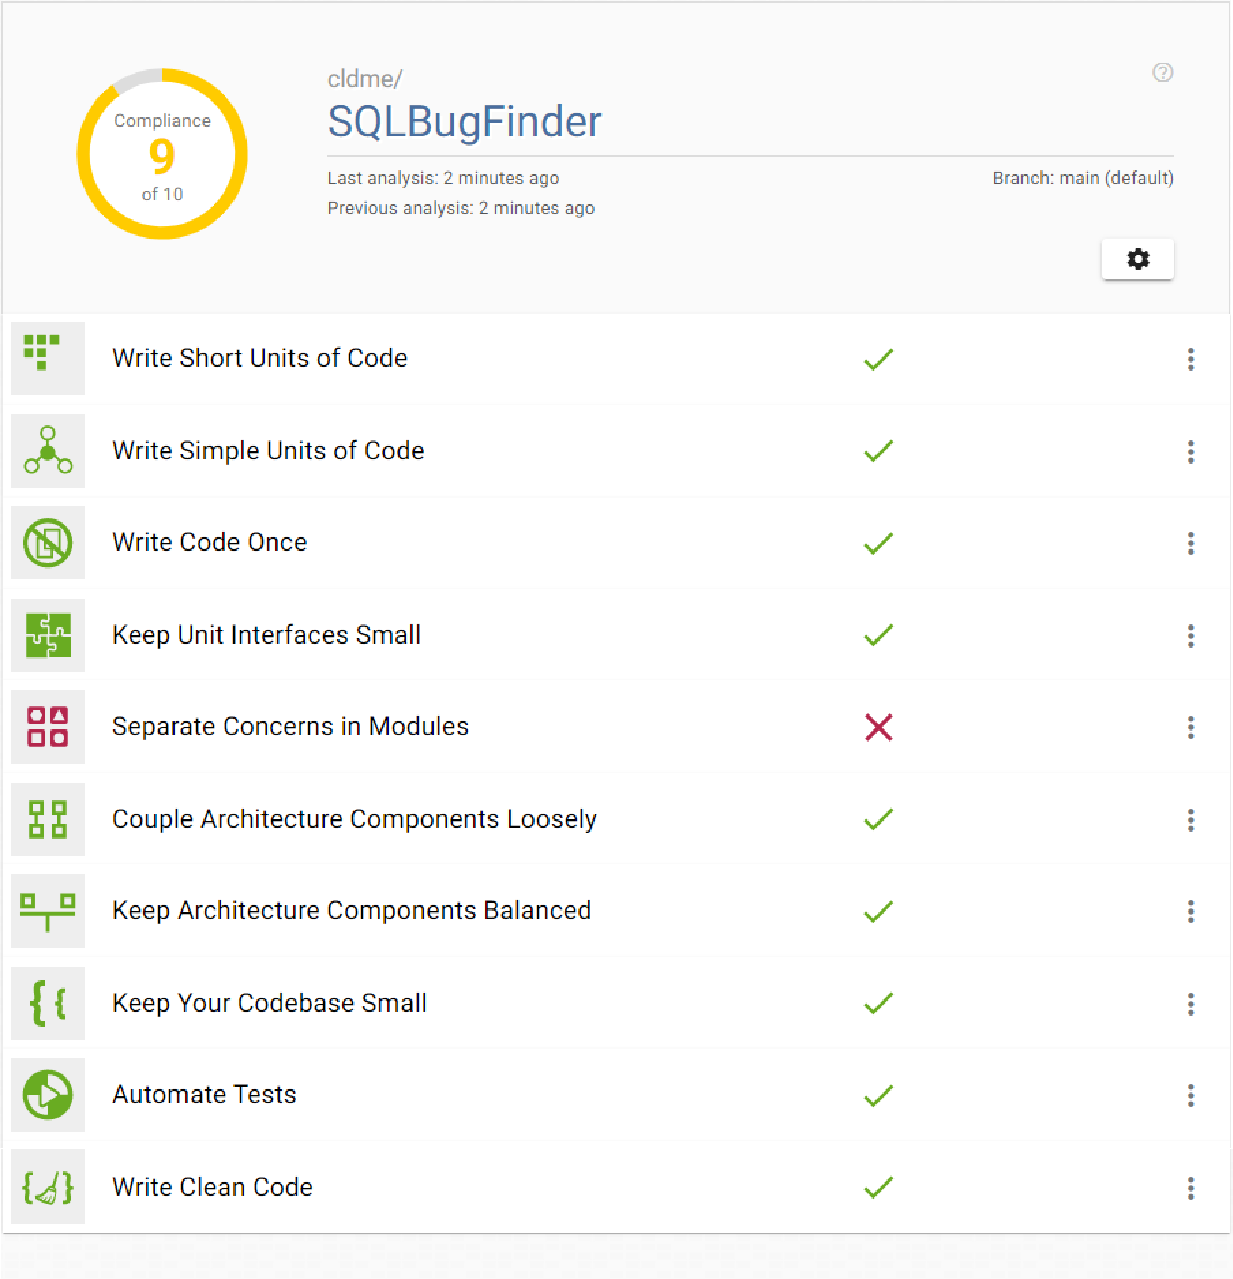
\includegraphics[width=0.95\textwidth]{img/code_hub.pdf}
    \caption{Code quality analysis}
    \label{fig:code_quality}
\end{figure}